\documentclass[14pt,aspectratio=1610]{beamer}
%\documentclass[12pt,aspectratio=1610,handout]{beamer}
\usepackage{csu-theme}
\usepackage{amsmath}
\usepackage{booktabs}

\usepackage{forest}
\forestset{
  default preamble={%
    for tree={%
      draw, % show border
      edge={-stealth, shorten >=1pt, shorten <=-1pt}, % show arrow to child
      edge=very thick, % edge weight
      very thick, % node border
      fill=CSUcyan, % node fill
      text=black,% text color
      fit=tight,% options: tight|rectangle|band
      inner ysep=0,
      inner xsep=1pt,
      minimum height=1.75em,
    },%
  },%
  %
  invalid/.style={%
    {fill=red!25}%
  },
  visible on/.style={
  for tree={
    /tikz/visible on={#1},
    edge+={/tikz/visible on={#1}}}}
}

\tikzset{
  %
  % Used for beamer overlays
  invisible/.style={opacity=0,text opacity=0},
  visible on/.style={alt=#1{}{invisible}},
  alt/.code args={<#1>#2#3}{%
    \alt<#1>{\pgfkeysalso{#2}}{\pgfkeysalso{#3}} % \pgfkeysalso doesn't change the path
  },
}

\NewDocumentCommand{\BTreeSep}{}{%
  {\color{fg}\rule[-0.5em]{1.25pt}{1.75em}}%
}

\NewDocumentCommand{\BTreeVal}{ sD<>{CSUcyan}m }{%
  \begingroup
  \setlength{\fboxsep}{5.5pt}% make the spacing wider to cover the whole cell
  \colorbox{#2}{\hspace{-5.5pt}\makebox[1.75em][c]{\vspace{1.5em}#3\vspace{1.5em}}\hspace{-5.5pt}}%
  \IfBooleanTF #1%
    {}%
    {\BTreeSep}%
  \endgroup
}

% \NewDocumentCommand{\BTreeNode}{ m }{%
%   \foreach \element in {#1} {%
%     \BTreeVal{\element}%
%   }%
% }

\NewDocumentCommand{\BTreeNode}{ m }{%
	\begingroup
	\foreach\element [count=\i from 1] in {#1} {%
		\ifnum\i>1%After the first element
      \BTreeSep%
		\fi%
      \makebox[1.75em][c]{\vspace{1.5em}\element\vspace{1.5em}}%
	}%
	\endgroup%
}

\title{\Huge{} B-Trees\\[-0.5em]{\Large{} External Memory Search}}
\subtitle{CSCI 315: Data Structure Analysis\\Chapter 14 of \href{https://opendatastructures.org/ods-cpp.pdf}{Open Data Structures}}
\author{Sean T. Hayes, Ph.D.}
\institute{Charleston Southern University}

%% Comment out date to use default (today)
% \date{April 3, 2025}
\subject{Software Programming}
%\keywords{}

\setlength{\parskip}{0.5em}

\graphicspath{{../imgs/}{../imgs/b-trees}}

\begin{document}

\begin{frame}
  \titlepage
\end{frame}

\section*{Intro}

\begin{frame}{Motivation for B-Trees}
\begin{itemize}[<+->]
  \item
    Index structures for large datasets cannot fit \\in main memory.
  \item
    Hard drive storage requires a different approach \\to efficiency.
  \item
    If a disk spins at 7,200 RPM, one revolution occurs in 1/120 of a second, or 8.33ms.
  \item
    One disk access takes more time than 200,000 instructions.
  \item
    One access on a modern SSD is approximately 2,500 times slower than reading from memory.
\end{itemize}
\end{frame}

\begin{frame}{Motivation for B-Trees}
\begin{itemize}[<+->]
  \item
    Suppose an \href{https://en.wikipedia.org/wiki/AVL_tree}{AVL tree} is used to store 20 million \\records.
  \item
    This very deep binary tree requires lots of different \\disk accesses;\\
    \(\log_2{20,000,000} \approx 24\), so this takes about 0.2 seconds.
  \item
    We know we can't improve on the \(\log_2{n}\) lower bound on the search for a binary tree.
  \item
    The solution is to use more branches and, thus, reduce the tree height!
  \begin{itemize}
    \item
      As branching increases, depth decreases.
  \end{itemize}
\end{itemize}
\end{frame}

\begin{frame}{Example B-Tree, Order-5 with 26 Elements}
  \begin{figure}
  \centering
  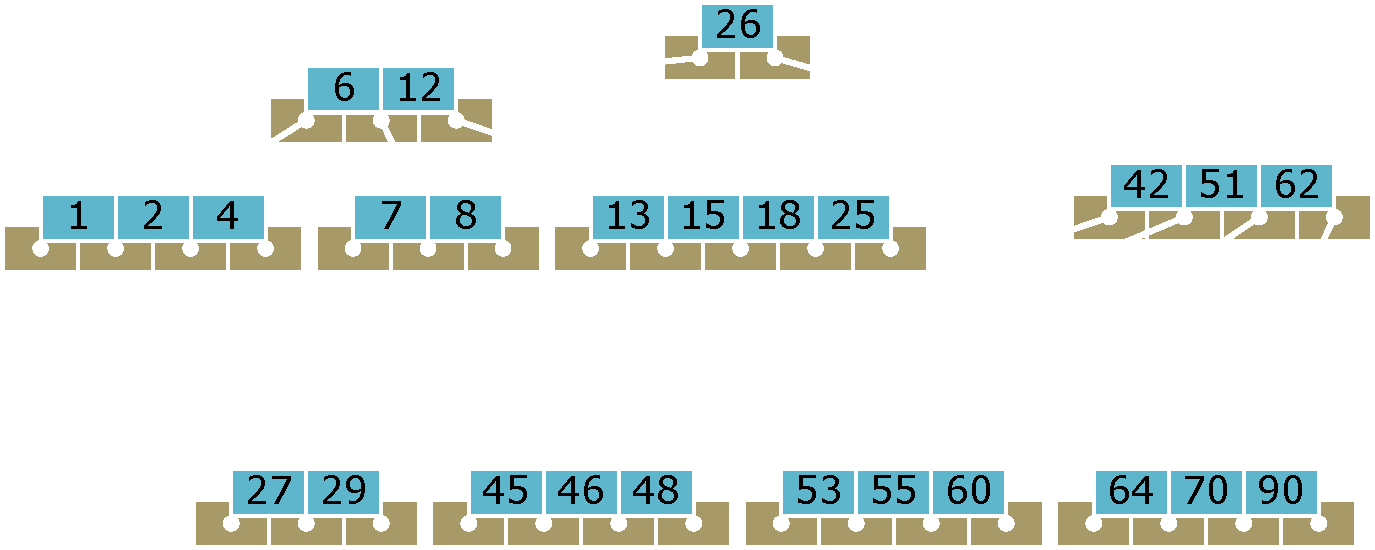
\includegraphics[width=\textwidth]{order-5-b-tree-example}
  \caption{Note that all the leaves are at the same level.}
  \end{figure}
\end{frame}

\begin{frame}{Definition of a B-tree}
  A B-tree of order \(m\) is an \(m\)-way tree (i.e., a tree where \\each node may have up to \(m\) children) in which:\pause{}

    \begin{enumerate}
      \item<+->
        All leaves are on the same level.
      \item<+->
        The number of children of a non-leaf node is always one more than the number of keys.
      \item<+->
        The keys of a node are sorted in increasing order. These keys partition the child keys as a search tree.
      \item<+->
        The root is either a leaf node or has two to \(m\) children.
      \item<+->
        Other non-leaf nodes have at least \(\left\lceil {m / 2} \right\rceil\) children.
      \item<+->
        A node contains no more than \(m - 1\) keys.
    \end{enumerate}
    \onslide<+->{The number \(m\) should always be odd.}
\end{frame}

\begin{frame}{Example B-Tree, Order-5 with 26 Elements}
\begin{figure}
\centering
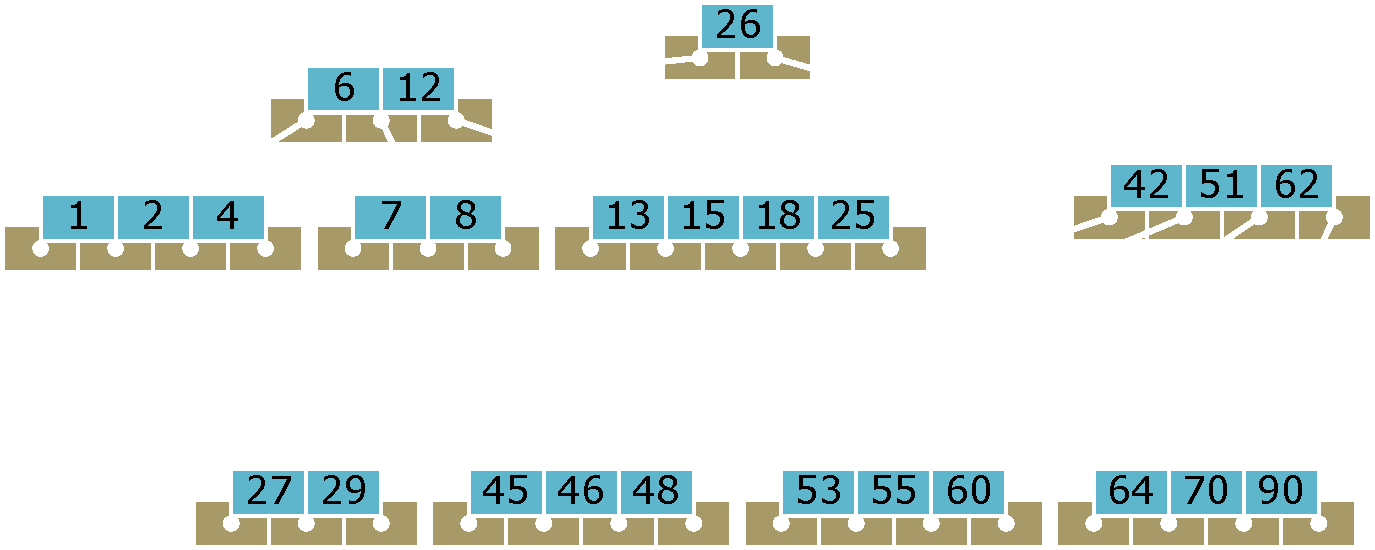
\includegraphics[width=\textwidth]{order-5-b-tree-example}
\caption{Note that all the leaves are at the same level.}
\end{figure}
\end{frame}

\section{Insert}

\begin{frame}[t]{Constructing a B-Tree}
Starting with an empty \emph{Order-5} B-tree, let's insert the \\following sequence of keys:\\
    1, 12, 8, 2, 25, 6, 14, 28, 17, 7, 52, 16, 48, 68, 3, 26, 29, 55, 45.
\begin{itemize}\small{}
  \item<2->
    The first four items go into the root:
    \begin{figure}
    \centering
    \begin{forest}
      [%
        \alt<-2>{%
          \BTreeNode{1}%
        }{%
          \alt<-3>{%
            \BTreeNode{1, 12}%
          }{%
            \alt<-4>{%
              \BTreeNode{1, 8, 12}%
            }{%
              \BTreeNode{1, 2, 8, 12}%
            }%
          }%
        }%
      ]%
    \end{forest}
    \onslide<5>{}
    \end{figure}
\end{itemize}
\end{frame}

\begin{frame}[t]{Constructing a B-Tree}
1, 12, 8, 2, \alert{\textbf{25}}, 6, 14, 28, 17, 7, 52, 16, 48, 68, 3, 26, 29, 55, 45.
\begin{itemize}\small{}
\item<1->
    Putting the fifth item in the root would violate condition 5.
    \begin{figure}
    \centering
      \begin{forest}
        [\BTreeNode{1, 2, 8, 12}\only<2->{\BTreeSep\BTreeVal*<red!75>{25}}]
      \end{forest}
    \end{figure}

  \item<3->
    Therefore, when 25 arrives, pick the middle key to make a new root.
    \begin{figure}
    \centering
      \begin{forest}
        [\BTreeVal*{8}
          [\BTreeNode{1, 2}]
          [\BTreeNode{12, 25}]
        ]
      \end{forest}
    \end{figure}
\end{itemize}
\end{frame}

\begin{frame}[t]{Constructing a B-Tree}
  1, 12, 8, 2, 25, \alert{\textbf{6, 14, 28}}, 17, 7, 52, 16, 48, 68, 3, 26, 29, 55, 45.
  \begin{itemize}\small{}
    \item<2->
      6, 14, and 28 get added to the leaf nodes.
  \end{itemize}

  \begin{figure}\small{}
  \centering
    \begin{forest}
      [\BTreeVal*{8}
        [
          \alt<-2>{%
            \BTreeNode{1, 2}%
          }{%
            \BTreeNode{1, 2, 6}%
          }%
        ]
        [
          \alt<-3>{%
            \BTreeNode{12, 25}%
          }{%
            \alt<-4>{%
              \BTreeNode{12, 14, 25}%
            }{%
              \BTreeNode{12, 14, 25, 28}%
            }%
          }%
        ]
      ]
    \end{forest}\onslide<5>{}
  \end{figure}
\end{frame}


\begin{frame}[t]{Constructing a B-Tree}
1, 12, 8, 2, 25, 6, 14, 28, \alert{\textbf{17}}, 7, 52, 16, 48, 68, 3, 26, 29, 55, 45.
\begin{itemize}\small{}
  \item
    Adding 17 to the right leaf node would over-fill it.
    \begin{figure}
    \centering
      \begin{forest}
        [\BTreeVal*{8}
          [
            \BTreeNode{1, 2, 6}
          ]
          [
            \BTreeNode{12, 14}\BTreeSep\only<2->{\BTreeVal<red!75>{17}}\BTreeNode{25, 28}%
          ]
        ]
      \end{forest}
    \end{figure}
  \item<3->
    So, the middle key is promoted (to the root), splitting the leaves.
    \begin{figure}
    \centering
      \begin{forest}
        [\BTreeNode{8, 17}
          [
            \BTreeNode{1, 2, 6}
          ]
          [
            \BTreeNode{12, 14}
          ]
          [
            \BTreeNode{25, 28}%
          ]
        ]
      \end{forest}
    \end{figure}
\end{itemize}
\end{frame}

\begin{frame}[t]{Constructing a B-Tree}
1, 12, 8, 2, 25, 6, 14, 28, 17, \alert{\textbf{7, 52, 16, 48}}, 68, 3, 26, 29, 55, 45.
\begin{itemize}\small{}
  \item
    We can now add 7, 52, 16, 48 to the leaf nodes.
    \begin{figure}
    \centering
      \begin{forest}
        [\BTreeVal{8}\BTreeVal*{17}
          [
            \BTreeNode{1, 2, 6}\alt<1>{}{\BTreeSep\BTreeVal*{7}}%
          ]
          [
            \BTreeNode{12, 14}\alt<-3>{}{\BTreeSep\BTreeVal*{16}}%
          ]
          [
            \BTreeNode{25, 28}\alt<-2>{}{\alt<-4>{}{\BTreeSep\BTreeVal*{48}}\BTreeSep\BTreeVal*{52}%
            }
          ]
        ]
      \end{forest}\onslide<5>{}
    \end{figure}
\end{itemize}
\end{frame}

\begin{frame}[t]{Constructing a B-Tree}
1, 12, 8, 2, 25, 6, 14, 28, 17, 7, 52, 16, 48, \alert{\textbf{68}}, 3, 26, 29, 55, 45.
\begin{itemize}\small{}
  \item
    Adding 68 to the right leaf node would over-fill it.
    \begin{figure}
    \centering
      \begin{forest}
        [\BTreeVal{8}\BTreeVal*{17}
          [
            \BTreeNode{1, 2, 6, 7}
          ]
          [
            \BTreeNode{12, 14, 16}
          ]
          [
            \BTreeNode{25, 28, 48, 52}\alt<1>{}{\BTreeSep\BTreeVal*<red!75>{68}}%
          ]
        ]
      \end{forest}
    \end{figure}
  \item<3->
    So we split the rightmost leaf, promoting 48 to the root.
    \begin{figure}
    \centering
      \begin{forest}
        [\BTreeNode{8, 17, 48}
          [
            \BTreeNode{1, 2, 6, 7}
          ]
          [
            \BTreeNode{12, 14, 16}
          ]
          [
            \BTreeNode{25, 28}
          ]
          [
            \BTreeNode{52, 68}
          ]
          [, phantom]
        ]
      \end{forest}
    \end{figure}
\end{itemize}
\end{frame}


\begin{frame}[t]{Constructing a B-Tree}
1, 12, 8, 2, 25, 6, 14, 28, 17, 7, 52, 16, 48, 68, \alert{\textbf{3}}, 26, 29, 55, 45.
\begin{itemize}\small{}
  \item
    Adding 3 to the left leaf node would over-fill it
    \begin{figure}
    \centering
      \begin{forest}
        [\BTreeNode{8, 17, 48}, for tree={l sep=1.5em, s sep=2em}
          [
            \alt<1>{%
              \BTreeNode{1, 2, 6, 7}%
            }{
              \BTreeNode{1, 2}\BTreeSep\BTreeVal<red!70>{3}\BTreeNode{6, 7}%
            }
          ]
          [
            \BTreeNode{12, 14, 16}
          ]
          [
            \BTreeNode{25, 28}
          ]
          [
            \BTreeNode{52, 68}
          ]
          [, phantom]
        ]
      \end{forest}
    \end{figure}
  \item<3->
    Adding 3 causes us to split the leftmost leaf, promoting 3 to the root.
    \begin{figure}
    \centering
      \begin{forest}
        [\BTreeNode{3, 8, 17, 48}, for tree={l sep=1.5em, s sep=2em}
          [
            \BTreeNode{1, 2}%
          ]
          [
            \BTreeNode{6, 7}%
          ]
          [
            \BTreeNode{12, 14, 16}
          ]
          [
            \BTreeNode{25, 28}
          ]
          [
            \BTreeNode{52, 68}
          ]
        ]
      \end{forest}
    \end{figure}
\end{itemize}
\end{frame}

\begin{frame}[t]{Constructing a B-Tree}
1, 12, 8, 2, 25, 6, 14, 28, 17, 7, 52, 16, 48, 68, 3, \alert{\textbf{26, 29, 55}}, 45.
\begin{itemize}\small{}
  \item
    26, 29, 55 then go into the leaves.
    \begin{figure}
    \centering
      \begin{forest}
        [\BTreeNode{3, 8, 17, 48}, for tree={l sep=2.2em, s sep=1em}
          [
            \BTreeNode{1, 2}%
          ]
          [
            \BTreeNode{6, 7}%
          ]
          [
            \BTreeNode{12, 14, 16}
          ]
          [
            \BTreeNode{25}\BTreeSep\only<2->{\BTreeVal{26}}\alt<-2>{\BTreeVal*{28}}{\BTreeNode{28, 29}}
          ]
          [
            \BTreeNode{52}\BTreeSep\only<4->{\BTreeVal{55}}\BTreeVal*{68}
          ]
        ]
      \end{forest}
    \end{figure}
\end{itemize}
\end{frame}

\begin{frame}[t]{Constructing a B-Tree}
1, 12, 8, 2, 25, 6, 14, 28, 17, 7, 52, 16, 48, 68, 3, 26, 29, 55, \alert{\textbf{45}}.
\begin{itemize}\small{}
  \item
    Adding 45 causes a split of the 4th leaf.\only<2->{\vspace{-1em}}
    \begin{figure}
    \centering
      \begin{forest}
        [\BTreeNode{3, 8, 17, 48}, for tree={l sep=2.2em, s sep=1em}
          [
            \BTreeNode{1, 2}%
          ]
          [
            \BTreeNode{6, 7}%
          ]
          [
            \BTreeNode{12, 14, 16}%
          ]
          [
            \BTreeNode{25, 26, 28, 29}%
              \only<2->{\BTreeSep\BTreeVal*<red!75>{45}}%
          ]
          [
            \BTreeNode{52, 55, 68}%
          ]
        ]
      \end{forest}
    \end{figure}
  \item<3->
    Promote 28 to the root, which causes the root to split.\vspace{-1em}
    \begin{figure}
    \centering
      \begin{forest}
        [\BTreeNode{3, 8, 17}\BTreeSep\BTreeVal<red!75>{28}\BTreeVal*{48}, for tree={l sep=2.2em, s sep=1em}
          [
            \BTreeNode{1, 2}%
          ]
          [
            \BTreeNode{6, 7}%
          ]
          [
            \BTreeNode{12, 14, 16}%
          ]
          [
            \BTreeNode{25, 26}
          ]
          [
            \BTreeNode{29, 45}%
          ]
          [
            \BTreeNode{52, 55, 68}%
          ]
        ]
      \end{forest}
    \end{figure}
\end{itemize}
\end{frame}

\begin{frame}[t]{Constructing a B-Tree}
1, 12, 8, 2, 25, 6, 14, 28, 17, 7, 52, 16, 48, 68, 3, 26, 29, 55, \alert{\textbf{45}}.
\begin{itemize}\small{}
  \item
    Promote 28 to the root; doesn't fit.
    \begin{figure}
    \centering
      \begin{forest}
        [\BTreeNode{3, 8, 17}\BTreeSep\BTreeVal<red!75>{28}\BTreeVal*{48}%, for tree={l sep=2.2em, s sep=1em}
          [
            \BTreeNode{1, 2}%
          ]
          [
            \BTreeNode{6, 7}%
          ]
          [
            \BTreeNode{12, 14, 16}%
          ]
          [
            \BTreeNode{25, 26}
          ]
          [
            \BTreeNode{29, 45}%
          ]
          [
            \BTreeNode{52, 55, 68}%
          ]
        ]
      \end{forest}
    \end{figure}
  \item<2->
    Promote the 17 as the new root.
    \begin{figure}
    \centering
      \begin{forest}
        [\BTreeNode{17}%, for tree={l sep=2.2em, s sep=1em}
          [\BTreeNode{3, 8}
            [
              \BTreeNode{1, 2}%
            ]
            [
              \BTreeNode{6, 7}%
            ]
            [
              \BTreeNode{12, 14, 16}%
            ]
          ]
          [
            \BTreeNode{28, 48}
            [
              \BTreeNode{25, 26}
            ]
            [
              \BTreeNode{29, 45}%
            ]
            [
              \BTreeNode{52, 55, 68}%
            ]
          ]
        ]
      \end{forest}
    \end{figure}
\end{itemize}
\end{frame}

\begin{frame}{Constructing a B-Tree}
\begin{itemize}[<+->]
  \item
    Attempt to insert the new key into a leaf.
  \item
    If this would result in that leaf becoming too big, split the leaf into two, promoting the middle key to the leaf's parent.
  \item
    If this would result in the parent becoming too big, split the parent into two, promoting the middle key.
  \item
    This strategy may need to repeat to the root.
  \item
    If necessary, the root is split in two and the middle key is promoted to a new root, making the tree one level higher.
\end{itemize}
\end{frame}

\begin{frame}{Exercise in Inserting a B-Tree }
\large
Insert the following keys to a 5-way B-tree:\\
3, 7, 9, 23, 45, 1, 5, 14, 25, 24, 13, 11, 8, 19, 4, 31, 35, 56, 2, 6, 12.
\end{frame}


\section{Remove}

\begin{frame}{Removal from a B-Tree}
  \center{}
Key are always inserted \emph{into leaves}.

For removal, we wish to remove \emph{from a leaf}.

There are four removal cases to consider in order.
\end{frame}

\begin{frame}{Cases for Removal from a B-Tree}
\begin{enumerate}
  \item<+->
    If the key is already in a leaf node and removing it\\
    doesn't cause that leaf node to have too few keys, \\
    then simply remove the key to be deleted.
  \item<+->
    If the key is \emph{not} in a leaf, then it is guaranteed (by the nature of a B-tree) that its predecessor and successor will be in leaves --- in this case, we can delete the key and promote the predecessor or successor key to the non-leaf deleted key's position.
\end{enumerate}
\end{frame}

\begin{frame}{Cases for Removal from a B-Tree}
If deleting a key in a leaf with the minimum key count or if Case (2) leads to a leaf node containing fewer than the minimum key count, then:

\begin{enumerate}
  \setcounter{enumi}{2}
  \item<2->
    If a sibling leaf has more than the min.\ number of keys, then we can promote one of its keys and move the parent key into the lacking leaf.
  \item<3->
    Otherwise, combine the lacking node and one of its neighbors with their shared parent (the opposite of promoting a key). The new node will have the correct number of keys. If the parent now has too few keys, repeat this case (up to the root itself if required).
\end{enumerate}
\end{frame}

\begin{frame}{Type 1: Simple Removal from Leaf}
Assuming a 5-way B-Tree (as before), \emph{delete 2}.\\

\begin{figure}
\centering
  \begin{forest}
    [\BTreeNode{12, 29, 52}, for tree={s sep=1.5em}
      [
        \alt<1>{\BTreeNode{2, 7, 9}}{\BTreeNode{7, 9}}
      ]
      [
        \BTreeNode{15, 22}
      ]
      [
        \BTreeNode{31, 43}
      ]
      [
        \BTreeNode{56, 69, 72}
      ]
    ]
  \end{forest}\onslide<2>{}
\end{figure}

Because there are enough keys in the node, just delete it.
\end{frame}

\begin{frame}{Type 2: Simple Removal from Non-Leaf}
Assuming a 5-way B-Tree (as before), \emph{delete 52}.\\

\begin{figure}
\centering
  \begin{forest}
    [\BTreeNode{12, 29, \alt<-2>{52}{56}}, name=root, for tree={s sep=1.5em}
      [
        \BTreeNode{7, 9}
      ]
      [
        \BTreeNode{15, 22}
      ]
      [
        \BTreeNode{31, 43}
      ]
      [
        \only<-3>{\BTreeVal{56}}\BTreeVal{69}\BTreeVal*{72}, name=rightLeaf
      ]
    ]
    \only<2-3>{
      \draw[->,dotted, very thick] ([xshift=1em]rightLeaf.north west) to[bend right] (root.east);
    }
  \end{forest}\onslide<4>{}
\end{figure}
Replace with the closest value from a leaf with enough values.
\end{frame}

\begin{frame}{Type 4: Too few keys in node and its siblings}
Delete 72

\begin{figure}
\centering
  \alt<-3>{
    \begin{forest}
      [ \BTreeVal{12}\alt<-3>{\BTreeVal{29}}{\BTreeVal*{29}}%
        \alt<-2>{%
          \BTreeVal*{56}%
        }{%
          \only<-3>{\BTreeVal*<CSUgold>{56}}%
        }, name=root, for tree={s sep=1.5em}
        [
          \BTreeNode{7, 9}
        ]
        [
          \BTreeNode{15, 22}
        ]
        [
          \alt<-2>{%
            \BTreeNode{31, 43}%
          }{%
            \alt<-3>{%
              \BTreeVal<CSUgold>{31}\BTreeVal*<CSUgold>{43}%
            }{%
              \BTreeNode{31, 43, 56, 69}
            }
          }
        ] {
          \only<3>{\draw[<-,CSUgold!50!white, very thick] ([xshift=0.75em] .south east)--++(0em,-1.5em)--++(-1em,0pt)
              node[anchor=east,align=center]{Join back together};}
        }
        [
          \alt<1>{%
            \BTreeNode{69, 72}%
          }{%
            \alt<-2>{%
              \BTreeVal*<red!75>{69}%
            }{%
              \only<3->{\BTreeVal*<CSUgold>{69}}%
            }%
          }, name=rightLeaf, visible on=<-3>
        ] {
            \onslide<2>{\draw[<-,red!50!white, very thick] (.south)--++(0em,-1.5em)--++(-1.5em,0pt)
            node[anchor=east,align=center]{Too few keys!};}
          }
      ]
    \end{forest}
  }{
    \begin{forest}
      [ \BTreeNode{12, 29}%
        [
          \BTreeNode{7, 9}
        ]
        [
          \BTreeNode{15, 22}
        ]
        [
          \BTreeNode{31, 43, 56, 69}
        ]{
          \onslide<2>{\draw[<-,red!50!white, very thick] (.south)--++(0em,-1.5em)--++(-1.5em,0pt)
          node[anchor=east,align=center]{This is just a placeholder};}
        }
      ]
    \end{forest}
  }
  \onslide<4>{}
\end{figure}
\end{frame}

\begin{frame}{Type 3: Enough siblings}
Delete 22

\begin{figure}
\centering
  \begin{forest}
    [ \BTreeVal{12}\alt<-3>{\BTreeVal*{29}}{\BTreeVal*{31}}, name=root%
      [
        \BTreeNode{7, 9}
      ]
      [
        \BTreeNode{15}\BTreeSep%
        \alt<1>{%
          \BTreeVal*{22}%
        }{%
          \alt<-3>{%
            \BTreeVal*<red!75>{\textcolor{red!75}{22}}%
          }{%
            \BTreeVal*{29}%
          }
        }
      ]{
          \onslide<2>{\draw[<-,red!50!white, very thick] (.south)--++(0em,-1.5em)--++(0.5em,0pt)
          node[anchor=west,align=center]{Too few keys!};}
          \onslide<3>{
              \draw[->,dotted, very thick] ([xshift=0.5em]root.south) to[bend right] ([xshift=1em].north);
            }
        }
      [
        \only<-3>{\BTreeVal{31}}\BTreeNode{43, 56, 69}
      ]{\onslide<3>{
            \draw[->,dotted, very thick] ([xshift=-3em].north) to[bend right=20] ([xshift=1.5em]root.south);
          }
        }
    ]
  \end{forest}\onslide<4>{}
\end{figure}
\end{frame}

\begin{frame}{Exercise in Removal a B-Tree }
\large
Given a 5-way B-tree created by these data (last exercise):\\
3, 7, 9, 23, 45, 1, 5, 14, 25, 24, 13, 11, 8, 19, 4, 31, 35, 56, 2, 6, 12\\[2em]

Delete these keys: 4, 5, 7, 3, 14, 45
\end{frame}

\section{Analysis}

\begin{frame}{Maximum Keys in an Order-\(m\) B-Tree}
  \begin{columns}
    \column{0.3\textwidth}%
    Max keys per level:\\
      \begin{tabular}{c c}
        \toprule
        Level & Key Count\\
        \midrule
      root    & $m - 1$\\
      $1$ & $m^1(m - 1)$\\
      $2$ & $m^2(m - 1)$\\
      $\vdots$ & \multicolumn{1}{c}{$\vdots$} \\
      $h$ & $m^h(m - 1)$\\
      \bottomrule
      \end{tabular}
  \column{0.7\textwidth}\pause{}
    So, the maximum number of items is:
    \begin{align*}\vspace{-1em}
      t &= (1 + m + m^2 + m^3 + \cdots + m^h)(m - 1)\\
        &= \frac{m^{h+1} - 1}{m - 1} (m - 1)\\
        &= m^{h+1} - 1
    \end{align*}
  \end{columns}\vspace{1em}
  \pause{}
  When $m = 5$ and $h = 2$, this gives $5^{2 + 1} - 1 = 125 - 1 = 124$.
% \end{itemize}
\end{frame}

\begin{frame}{Big-$O$ of B-Trees}

{\center{}
\begin{table}
  \begin{tabular}{l l l}
    \toprule
      \textbf{Operation} & \textbf{Balanced Binary Tree} & \textbf{\(m\)-Way B Tree}\\
    \midrule
      Insert   & \onslide<2->{\(O(\log_2{n})\)} & \onslide<5->{\(O(\log_2{n})\)} \\
      Find     & \onslide<3->{\(O(\log_2{n})\)} & \onslide<6->{\(O(\log_2{n})\)} \\
      Delete   & \onslide<4->{\(O(\log_2{n})\)} & \onslide<7->{\(O(\log_2{n})\)} \\
    \bottomrule
  \end{tabular}
\end{table}
}
\vspace{1em}
\onslide<8->{
  The benefits are:
  \begin{enumerate}
    \item 
      Reduced hard-drive access (but the same number of instructions) and 
    \item 
      Reduced memory usage (fewer pointers).
  \end{enumerate}
}
\end{frame}

\begin{frame}{Reasons for Using B-Trees}

When searching tables held on a hard drive, the cost \\
of each drive transfer is high but doesn't depend much \\
on the amount of data transferred, especially if \\consecutive items are transferred.

\begin{itemize}
    \item
      For example, an order 101 B-tree can transfer each node in one drive read operation.
    \item
      An order 101 B-tree and height 3 can hold $101^4 - 1$ items (approximately 100 million) and any item can be accessed with 3 drive reads (assuming we hold the root in memory).
\end{itemize}
\end{frame}

\begin{frame}{Reasons for Using B-Trees}
If we take \(m = 3\), we get a \emph{2--3 Tree}, in which non-leaf nodes have two or three children (i.e., one or two keys).
\begin{itemize}
  \item
    B-Trees are always balanced (since the leaves are all at the same level), so 2-3 Trees make a good type of balanced tree.
\end{itemize}
\end{frame}

\begin{frame}{Comparing Trees}
\begin{itemize}[<+->]\large
  \item
    Binary trees
    \begin{itemize}
      \item
        Can become \emph{unbalanced} and lose their good time \\complexity (Big $O$).
      \item
        \emph{AVL Trees} are strict binary trees that \emph{overcome the balance problem}.
      \item
        Heaps remain balanced but are unsorted.
    \end{itemize}
  \item
    Multi-way trees
    \begin{itemize}
      \item
        B-Trees are \(m\)-way, with any (odd) number of children.
      \item
        The 3-Way B-Tree (a.k.a 2--3 Tree) approximates a self-balancing binary tree, exchanging the AVL tree's balancing operations for insertion and (more complex) deletion operations.
    \end{itemize}
\end{itemize}
\end{frame}

\section*{Name}
\begin{frame}{What does the ``B'' in B-Tree stand for?}
  \pause{}
  \begin{itemize}[<+->]
    \item
      No one knows.
    \item
      The inventors of the B-Tree will not say what it means.
    \item
      It could mean: Boeing (where it was invented), balanced, between, broad, bushy, and Bayer (the inventors are Bayer and McCreight).
    \item
      ``The more you think about what the `B' in B-trees means, the better you understand B-trees.''\\
      \hspace{1em}--- Edward M. McCreight (2013)
  \end{itemize}
  \end{frame}

\section*{Lab 21}
\begin{frame}{Lab 20: B-Trees}
\begin{center}\Large
  Let's look at the lab based on today's lecture.
\end{center}
\end{frame}
\end{document}